\section{Effects of Opacities on the Red Giant Branch Bump}
In addition to models of multiple populations in NGC 2808, we also have access
to GS98 solar composition models using OPAL and Ferguson opacities as well as
models using OPLIB and Aesopus opacities (high and low temperature
respectivley). Given the RGB bumps sensititvity to convective zone depth, as
demonstrated in the previous section, it is reasonable to assume that
variations in the opacity may have an effect on its location. 

Following the procedue outlined in \citep{Joyce2015} we identify the RGB Bump
in models evolved over a variety of [Fe/H]. All models use a GS98 solar
composition, high temperature opacities from OPLIB and low temperature
opacities from Aesopus. These are queried in the same manner as they were for
populations A and E in NGC 2808. Models are evolved with a typical numerical
tolerance of one part in 10$^{5}$ and include gravitational settling. 

The evolutionary tracks for each model are bolometrically corrected into
UBV(RI)c filters using the bolometric correction tables provided by MESA
\addcite and \fidanka. These bolometric corrections additionally assume $\mu =
0$ and $A_{v} = 0$. The magnitude of the bump is then defined as the magnitude
at the age where the magnitude-age derivitive is maximized. We visually inspect
all models to confirm that the identified magnitude aligns with the location of
the bump.

Comparing bump locations between OPAL+Ferguson opacities (Figure
\ref{fig:OPALvsOPLIBRGBB}) to OPLIB+Aesopus opacities we find that indeed the
updated opacities to effect the location of the bump; however, this is a very
small effect, on the order of a few parts in 100.

\begin{figure}
  \centering
  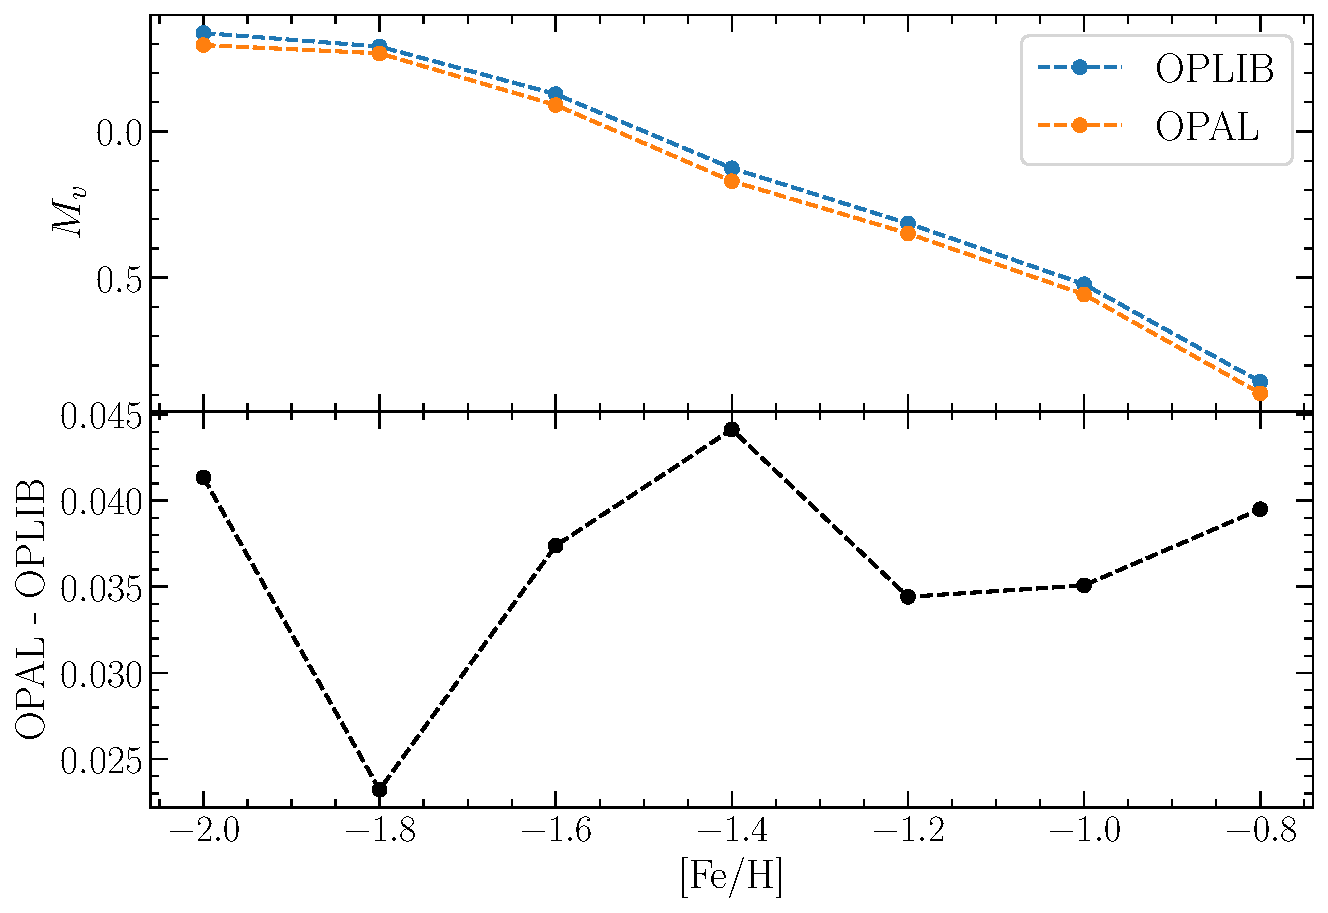
\includegraphics[width=0.85\textwidth]{figures/rgbb/OPALvsOPLIBComparison.pdf}
  \caption{V magnitude of the red giant branch bump as predicted by models
  evolved with OPAL+Ferg opacities and models evolved with OPLIB+Aesopus
  opacities. The updated opacities tend to push the bump to slightly smaller
  magnitudes; however, this is a very weak effect.}
  \label{fig:OPALvsOPLIBRGBB}
\end{figure}
